\documentclass[11pt, a4paper]{article}

\usepackage{graphicx}
\usepackage[a4paper,top=3cm,bottom=2cm,left=2cm,right=2cm,marginparwidth=1.75cm]{geometry}
\usepackage[english]{babel}
\usepackage[utf8x]{inputenc}
\usepackage{subfig}
\usepackage{amsmath}
\usepackage{amssymb}
\usepackage{cancel}

\graphicspath{ {./images} }
\newcommand*{\qed}{\hfill\ensuremath{\quad\square}}%
\newcommand*{\rad}{\ensuremath{\,\text{rad}}}
\newcommand*{\R}{\ensuremath{\mathbb{R}}}

\makeatletter
\renewcommand*\env@matrix[1][*\c@MaxMatrixCols c]{%
  \hskip -\arraycolsep
  \let\@ifnextchar\new@ifnextchar
  \array{#1}}
\makeatother

\newtheorem{theorem}{Theorem}

%------------------------------------------------
%Templates for images and figures
% \begin{figure}[h]
%   \centering
%   \subfloat[caption 1]{{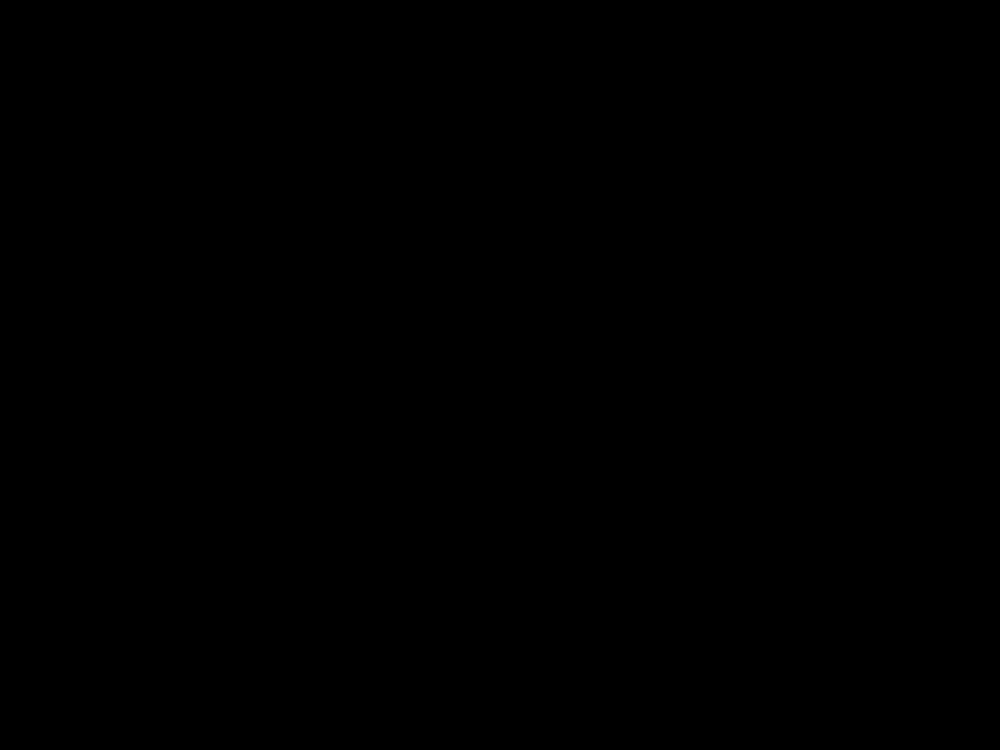
\includegraphics[width=30mm]{images/placeholder.png}}}%
%   \qquad
%   \subfloat[caption 2]{{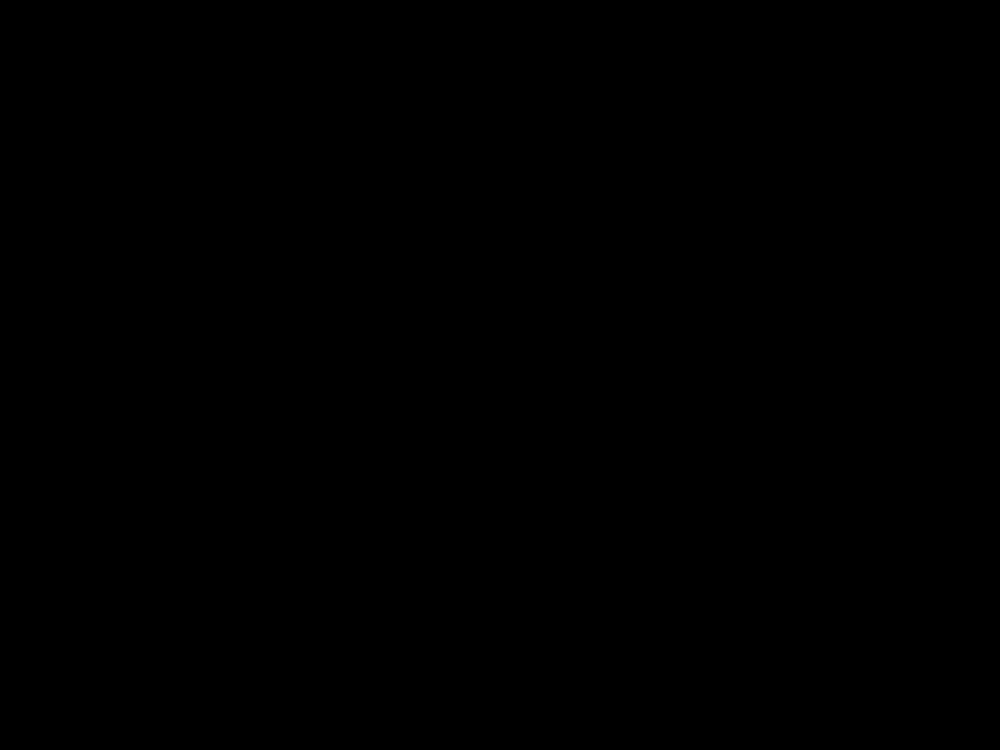
\includegraphics[width=30mm]{images/placeholder.png}}}%
%   \caption{Description}
% \end{figure}

% \begin{figure}[h]
%   \centerline{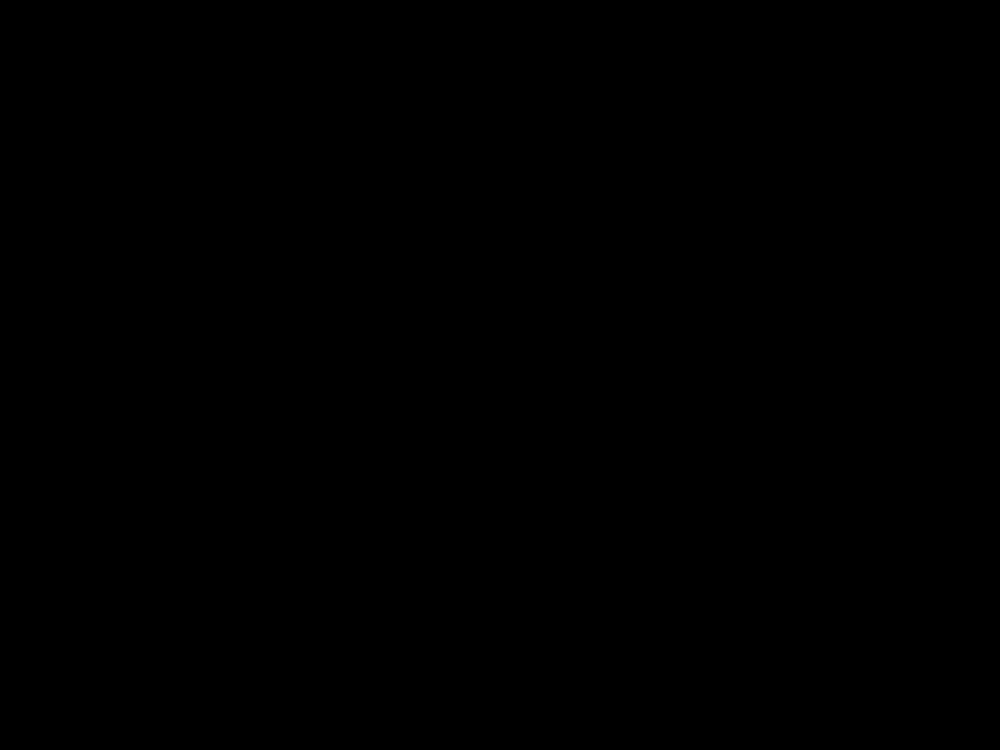
\includegraphics[width=50mm]{images/placeholder.png}}
%   \caption{Description}
% \end{figure}
%-----------------------------------------------

\begin{document}
\setcounter{section}{2}
\setcounter{equation}{0}
\section{Thermofluids Lecture 3: First law of thermodynamics (Part 2) (27/04/2020)}


\subsection{Quick recap of previous lecture}
The first law of thermodynamics is for a closed system is:
\begin{equation}
  \Delta KE + \Delta PE + \Delta U = Q - W
\end{equation}
Where $\Delta KE + \Delta PE + \Delta U = \Delta E$, $Q$ is energy transfer by heat ($Q > 0$ is transfer \underline{to} the system and $Q < 0$ is transfer \underline{from} the system.) and $W$ is energy transfer by work ($W > 0$ is work done \underline{by} the system and $W < 0$ is work done \underline{on} the system.).
The first law can also differently be denoted by any of the following expression:
\begin{itemize}
  \item Delta form: $\Delta E = \int_1^2 \delta Q - \int_1^2 \delta W = Q_{12} - W_{12}$
  \item Differential form: $dE = \delta Q - \delta W$
  \item Differential form per unit mass: $de = \delta q - \delta w$
  \item Differential form per unit time: $\frac{dE}{dt} = \dot{Q} - \dot{W}$
\end{itemize}


\subsection{The general procedure for solving thermodynamics problems}
\begin{enumerate}
  \item Sketch the system to be analyzed
  \item Indicate the system boundary
  \item List the made assumptions
  \item Indentify the reference fram (or datum, basicly the 0 reference point)
  \item Define the forces acting on the system
  \item Indicate the energy transfer by heat
  \item Indentify if the system is on a time interval or rate of change
\end{enumerate}

\begin{table}[h!]
  \begin{center}
    \caption{Internal energies for closed systems}
    \label{tab:table1}
    \begin{tabular}{l|c|c}
      \textbf{ } & \textbf{System} & \textbf{$\Delta U$}\\
      \hline
      diabatic & 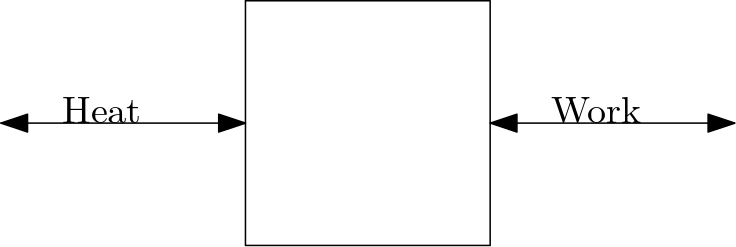
\includegraphics[ width=30mm]{images/Closed_diabatic.png}
               & $\Delta U = Q - W$\\
      
      adiabatic&\qquad \enspace 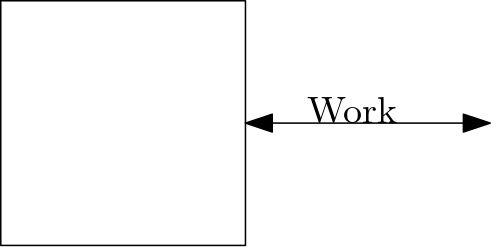
\includegraphics[ width=20mm]{images/Closed_adiabatic.png}
               & $\Delta U =\cancelto{0}{Q} - W$\\

      isolated &\includegraphics[ width=10mm]{images/isolated.png} & $\Delta U = \cancelto{0}{Q} - \cancelto{0}{W}$\\
    \end{tabular}
  \end{center}
\end{table}


\subsection{Modes of heat transfer}
There are 4 ways of transferring heat. These are as follows:
\begin{enumerate}
  \item Advection, Transport via a fluid which is dependent on the motion and momentum of the fluid (not covered)
  \item Conduction or diffusion, Transfer between objects in physical contact
  \item Radiation, Transfer by admission of electromagnetic radiation
  \item Convection, Transfer between an object and it's enviroment
\end{enumerate}
\underline{Conduction:}
Conduction is the transfer of heat between objects which are in physical constant with each other. Some materials conduct heat better then others (Copper and aluminium make great heat conducters while air sucks.) and thus the rate of transfer is proportional to some constant $\kappa$. Note the minus sign in the equation as heat is typically leaving the system via conduction.
\begin{equation}
  \dot{Q}_x = -\kappa A \frac{dT}{dx}
\end{equation}
Where $\kappa$ is the material's heat conductivity in $W/mK$. $A$ the surface area in contact and $\frac{dT}{dx}$ the one dimensional temperature gradient in the $x$ direction. For simple systems this can be assumed as linear over the thickness of a wall leading to $\frac{dT}{dx} = \frac{T_2 - T_1}{L}$ where $L$ is the wall thickness. Note that this is a one dimensional version of Fourrier's law. Which is more generally given as $\vec{\phi}_q = -\kappa \nabla T$, where $\vec{\phi}_q$ is the heat flux density in $W/m^2$.\\
\\
\underline{Radiation:}
Radiation is the loss of heat through electromagnetic radiation generated by the thermal motion of particles in matter. It's proportional to the emissivity of a material which is a value that describes how effective a given material is at radiating heat from it's surface. A material with an emissivity of $1$ would be considered a black body. The thermal radiation is also proportional to the amount of area radiating heat, the boltzmann constant and the temperature to a power of $4$.
\begin{equation}
  \dot{Q}_e = \epsilon \sigma A \Delta T^4
\end{equation}
$\epsilon$ is the emissivity of a given body (dimensionless), $\sigma$ is the Stefan-Boltzmann constant in $W/m^2K^4$ (The value of the constant is $5.67(10^{-8})\,W/m^2K^4$), $A$ the radiating area and $\Delta T$ the difference in temperature between the body and it's surroundings. For a given body considered in thermodynamics $\Delta T^4 = T_b^4 - T_s^4$ where $T_b$ is the temperature of the body and $T_s$ the temperature of the surroundings.\\
\\
\underline{Convection:}
Technically not really a mode of heat transfer as it is a combination of multiple other methods of heat transfer (Mainly advection and conduction). Nonetheless convection refers to the process of transferring heat from one place to another by the movement of fluids.
\begin{equation}
  \dot{Q}_c = hA(T_b - T_f)
\end{equation}
Note that this is basically Newton's law of cooling. $h$ is the heat transfer coefficient depending on the material and with the unit of $W/m^2K$, $A$ is the amount of contact area between the fluid and the body, $T_b$ is the temperature of the body and $T_f$ is the temperature of the fluid. 


\subsection{thermodynamic cylcles}
A thermodynamic cylce is a process which begins and ends at the same state. Examples of cycles are power cycles (developing a net energy transfer by work) and heat pump/refrigeration cycles (developing a net heat transfer of energy by inputting work.). An example of a thermodynamic power cycle is shown in figure 1.
\begin{figure}[h]
  \centerline{\includegraphics[width=50mm]{images/Power_Cycle.png}}
  \caption{An example of a $p,V$-diagram for a power cycle}
\end{figure}
\begin{align}
  \text{process } 1 \to 2:\; &U_2 - U_1 = Q_{12} - W_{12}\\
  \text{process } 2 \to 3:\; &U_3 - U_2 = Q_{23} - W_{23}\\
  \text{process } 1 \to 3:\; &U_2 - U_1 + U_3 - U_2 = (Q_{12} + Q_{23}) - (W_{12} + W_{23})\\
                             &U_1 = U_3 \Rightarrow Q_{12} + Q_{23} = W_{12} + W_{23}\\
                             &Q_{cycle} = W_{cycle}
\end{align}
Since for this process $W_{12} < 0$ and $W_{23} > 0$ there is a net gain in work (Also note that $|W_{12}| < |W_{23}|$). Because of this, this process is a power cycle.
The flow of energy for thermodynamic cylces is show in the figures 2 (a) and (b).
\begin{figure}[h]
  \centering
  \subfloat[Power cycle]{{\includegraphics[width=40mm]{images/energy_flow_powercycle.png}}}%
  \qquad
  \subfloat[Cooling/Heating cycle]{{\includegraphics[width=40mm]{images/energy_flow_heatcycle.png}}}%
  \caption{A visualization of cycle processes.}
\end{figure}


\subsection{Thermal efficiency and the COP}
Thermal efficiency and the COP are a way of mathematically expressing the amount of required input to get a desired output. It can thus be thought of as the "losses" in a given system. Note that these are not actual losses of energy, but rather energy being transformed or transfered in undesirable ways for a given output (e.g. creation of heat through friction when moving an object). Efficiency denoted as $\eta$ is defined as follows:
\begin{equation}
  \eta = \frac{\text{Desired output}}{\text{Required input}}
\end{equation}
Using this equation and figure 2 (a) we can express the thermal efficiency of a power cycle as:
\begin{equation}
  \eta_{th} = \frac{W_{cycle}}{Q_{net}}
\end{equation}
When describing the efficiency of a cooling or heating cycle we instead talk about a coefficient of performance. Much like efficiency, this is the ratio between the desired output and required output, where the output in the net heating or cooling. Note that for cooling the letter $\beta$ is used and for heating the letter $\gamma$. 
\begin{gather}
  \beta = \frac{\text{Cooling effect}}{\text{Work input}} = \frac{Q_{L}}{W_{net,in}}\\
  \gamma = \frac{\text{Heating effect}}{\text{Work input}} = \frac{Q_{H}}{W_{net,in}}
\end{gather}


\subsection{Example problem of a cyclical process}
A gas undergoes a thermodynamic cycle consisting of the following processes:
\begin{itemize}
  \item process $1 \to 2$: $p(V) = p$, $p = 1.4\,bar$, $V=0.028\,m^3$, $W_{12}=10.5\,kJ$
  \item process $2 \to 3$: Compression with $p(V) = \frac{k}{V}$, $U_3 = U_2$
  \item process $3 \to 1$: $V = $ constant, $U_1 - U_3 = -26.4\, kJ$
\end{itemize}
There are no significant changes in potential and kinetic energy. The $p,V$-diagram for the process is show in figure 3.
\begin{figure}[h]
  \centerline{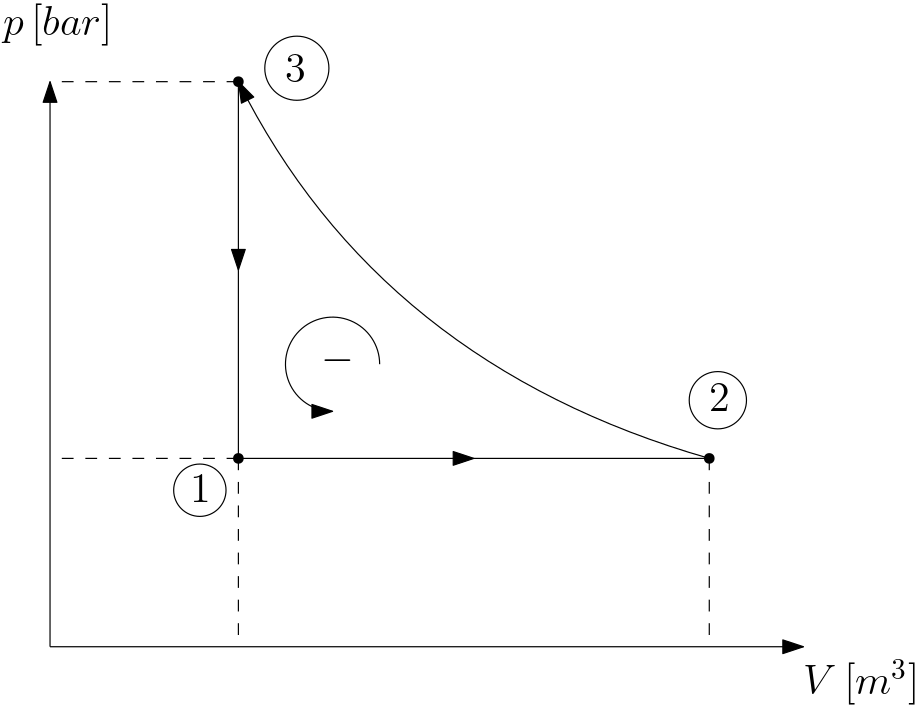
\includegraphics[width=50mm]{images/Example_process_cycle.png}}
  \caption{The $p,V$-diagram of the process described}
\end{figure}
From here we can create tables for the state and process variables:
\begin{table}[h!]
  \begin{center}
    \caption{A table for the process variables (Computations below)}
    \label{tab:table1}
    \begin{tabular}{l|r|r}
      \textbf{Process} & $Q\;[kJ]$ & $W\;[kJ]$\\
      \hline
      $1 \to 2$& 36.9 & 10.5\\
      
      $2 \to 3$& -18.78 & -18.78\\

      $3 \to 1$& -26.4 & 0\\
    \end{tabular}
  \end{center}
\end{table}
\begin{table}[h!]
  \begin{center}
    \caption{A table for the state variables (Computations below)}
    \label{tab:table1}
    \begin{tabular}{l|r|r}
      \textbf{State} & $p\;[\text{bar}]$ & $V\;[m^3]$\\
      \hline
      $1$ & 1.4 & 0.028\\
      
      $2$ & 1.4 & 0.103\\

      $3$ & - & 0.028\\
    \end{tabular}
  \end{center}
\end{table}
\begin{gather}
  \text{process $1 \to 2$:} \notag\\
  W_{12} = \int_1^2 p\,dV = p\cdot \int_1^2 dV = p(V_2 - V_1)\\
  V_2 = \frac{W_{12}}{p} + V_1 = 0.103\,m^3
\end{gather}
\begin{gather}
  \text{process $2 \to 3$:} \notag\\
  W_{23} = \int_2^3 p\,dV = k \cdot \int_1^2 \frac{1}{V}dV = k\cdot \ln\left(\frac{V_3}{V_2} \right) = -18.78\,kJ\\
  \cancelto{0}{\Delta U} = Q_{23} - W_{23} \Rightarrow Q_{23} = W_{23} = -18.78\,kJ
\end{gather}
\begin{gather}
  \text{process $3 \to 1$:} \notag\\
  \Delta U = Q_{31} - \cancelto{0}{W_{31}}\\
  U_1 - U_3 = Q_{31} = -26.4\,kJ
\end{gather}


\end{document}